\section{Idealidade dos gases}
	
\subsection{Determinação das constantes a e b na equação de Van Der Walls}

A equação dos gases ideais determina o comportamento de gases considerados ideais. O gás ideal é um modelo teórico, que se considera nula a interação entre as moléculas do gás. A equação é definida como:

$$\Large PV=nRT$$

Onde $P$ é a pressão absoluta,  $V$ é o volume do gás,  $n$ é o número de moles, $R$ constante universal dos gases e $T$ é a temperatura que o gás se encontra. 

Na prática sabe – se que as interações entre as moléculas de um gás são consideráveis, mas existem intervalos de pressão e temperatura em que alguns gases se aproximam do comportamento de um gás ideal (uns mais que outros) e essa equação é válida.

Uma equação alternativa a equação dos gases ideais é a equação de Van der Waals proposta por J.D. van der Waals em 1873:

$$\Large (P + \frac{a}{v^{2}} )(v-b)=RT$$

Nesse modelo proposto, $a$ e $b$ são constantes empíricas e $v$ é o volume molar do gás $(\large v=\frac{V}{n})$. A constante $a$ representa a intensidade das interações atrativas entre as partículas do gás e $b$ representa a intensidade das interações repulsivas. Essas constantes são características de cada gás e independem da temperatura.

Em projetos de engenharia envolvendo gases é, frequentemente, necessário determinar o volume que determinado número de moles de um gás ocupa a uma determinada pressão e temperatura. 
Vamos determinar o volume molar dos gases $N_{2}$ e $NH_{3}$ e comparar com o volume de um gás ideal calculado a partir da equação do gás ideal.

\begin{minted}{Scilab}
function raiz(xo, erro, iter_max, a, b, temp, P)  

// escreva aqui a equação que vc deseja determinar a raiz
function W = f(x) 
W = (P + a/(x^2))*(x - b) - 0.082054*temp
endfunction
// informe aqui a derivada da (função acima)
// em relação a varíavel dependente acima
function deriv = f_linha(x) 
deriv = P - (a/x^2) + (2*a*b)/x^3
endfunction
i = 1
X(i) = xo
// Quando o erro relativo for menor que
// o erro fornecido pelo usuário o loop é quebrado
while (2>1) 
// equação de Newton Raphson
X(i+1) = X(i) - (f(X(i))/f_linha(X(i))) 
if abs((X(i+1) - X(i))/X(i+1)) < erro
break
elseif i > iter_max
break
end
i = i+1
end   
printf("volume molar do gás com a equação de van der waals:")
disp(X(i))   
endfunction
// calcula o volume molar do gás ideal
function gas_ideal(P, T)
// 0.082054 é a constante universal dos gases R
vol = (0.082054*T)/P 
printf("Volume molar considerando gás como ideal:")
disp(vol)
endfunction 
\end{minted}

\begin{figure}[H]
	\centering
	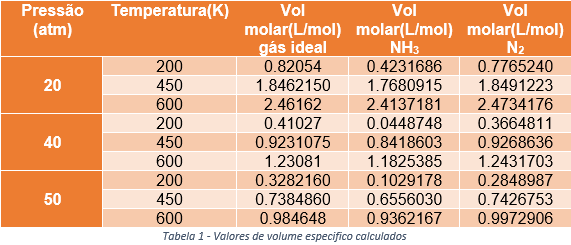
\includegraphics[width=0.8\textwidth]{./Imagens/Idealidade/ide1.png}
	\caption{Tabela dos gases}
	\label{fig:OHS1}
\end{figure}